% PRISMA Flow Diagram for SoK: Architectural and Economic Ceilings of Client-Side Anti-Automation
% Compiled with: pdflatex or lualatex
% Requires: tikz package
\documentclass[tikz,border=10pt]{standalone}
\usepackage{tikz}
\usetikzlibrary{shapes.geometric, arrows, positioning, fit, backgrounds, calc}

\begin{document}
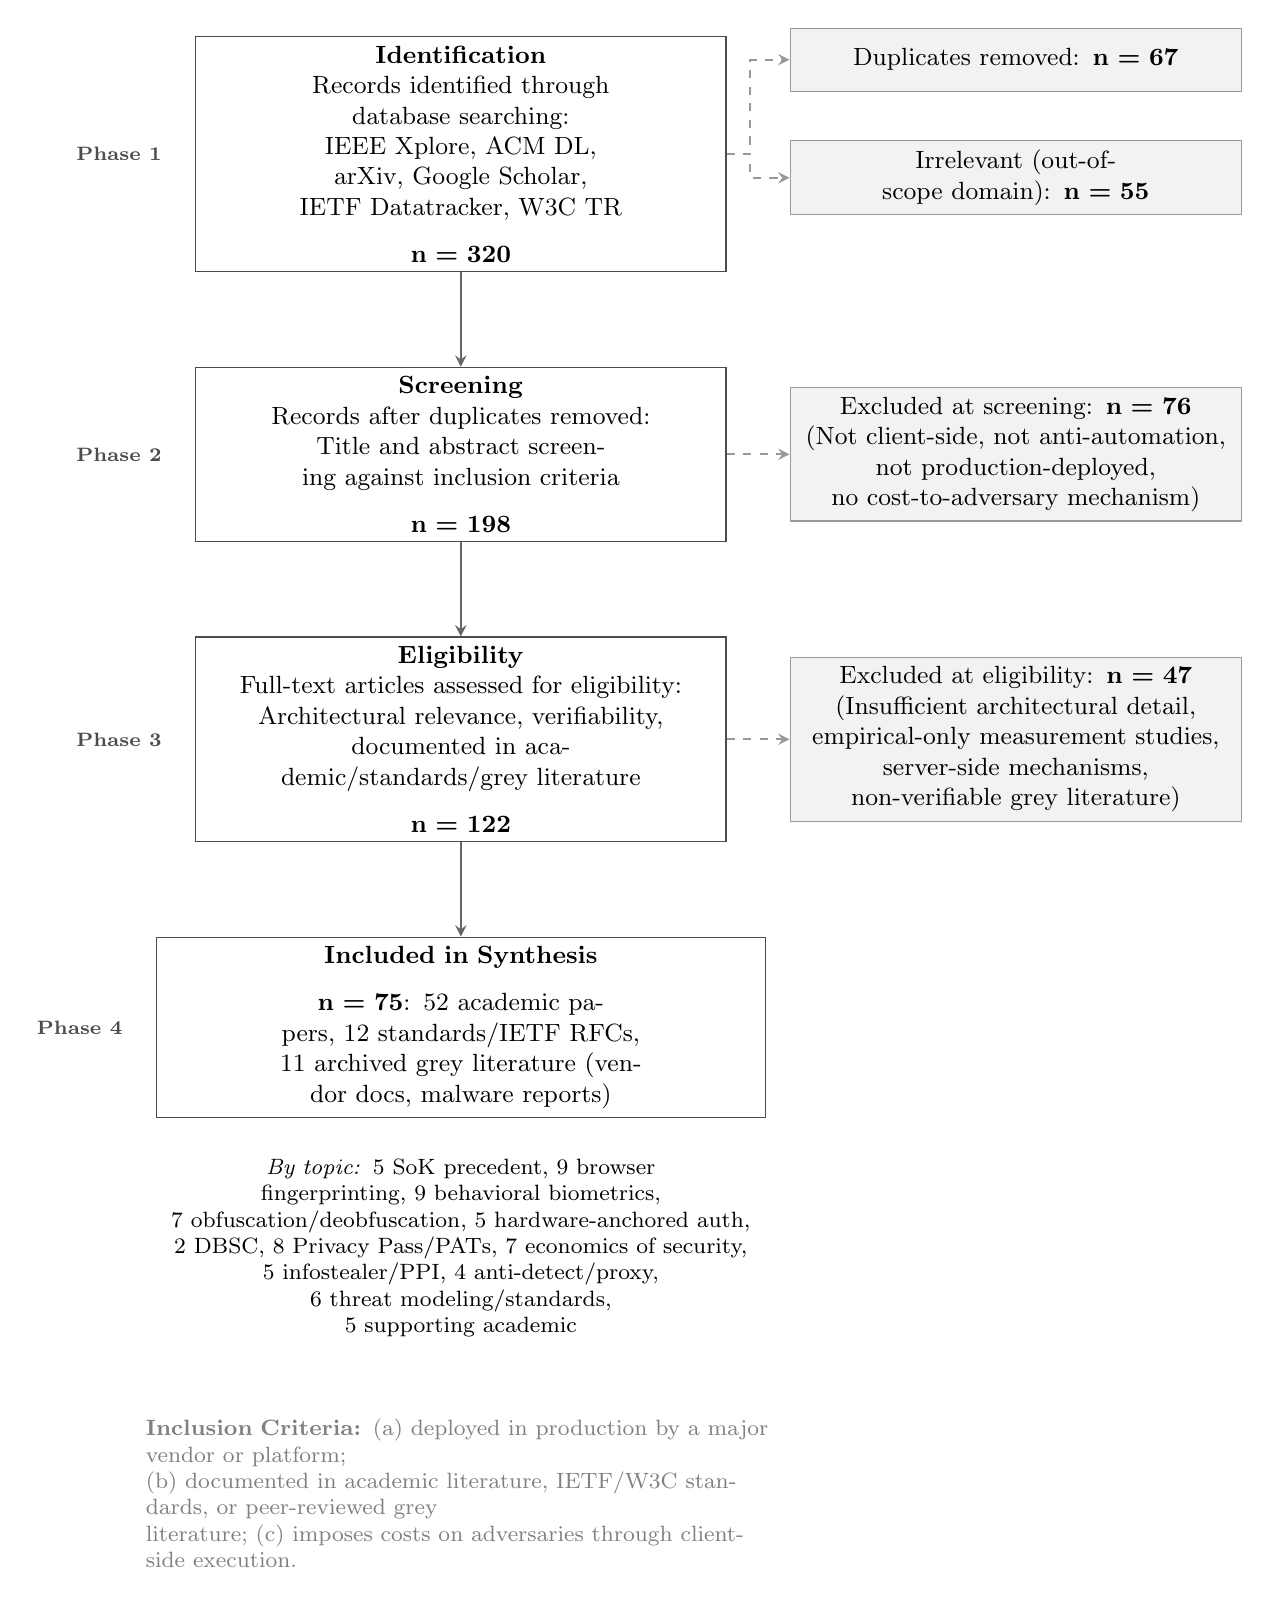
\begin{tikzpicture}[
    node distance=1.2cm,
    box/.style={
        rectangle,
        draw=black!70,
        fill=white,
        text width=6.5cm,
        align=center,
        minimum height=1.0cm,
        font=\small
    },
    excluded/.style={
        rectangle,
        draw=black!40,
        fill=black!5,
        text width=5.5cm,
        align=center,
        minimum height=0.8cm,
        font=\small
    },
    arrow/.style={
        ->,
        >=stealth,
        thick,
        black!60
    },
    label/.style={
        font=\scriptsize\bfseries,
        text=black!70
    }
]

% IDENTIFICATION box
\node[box] (identify) {
    \textbf{Identification} \\
    Records identified through database searching: \\
    IEEE Xplore, ACM DL, arXiv, Google Scholar, \\
    IETF Datatracker, W3C TR \\
    \medskip
    \textbf{n = 320}
};

% Excluded at identification
\node[excluded, right=0.8cm of identify, yshift=1.2cm] (excl-dup) {
    Duplicates removed: \textbf{n = 67}
};
\node[excluded, right=0.8cm of identify, yshift=-0.3cm] (excl-irrelevant) {
    Irrelevant (out-of-scope domain): \textbf{n = 55}
};

% SCREENING box
\node[box, below=of identify] (screen) {
    \textbf{Screening} \\
    Records after duplicates removed: \\
    Title and abstract screening against inclusion criteria \\
    \medskip
    \textbf{n = 198}
};

% Excluded at screening
\node[excluded, right=0.8cm of screen] (excl-screen) {
    Excluded at screening: \textbf{n = 76} \\
    (Not client-side, not anti-automation, \\
    not production-deployed, \\
    no cost-to-adversary mechanism)
};

% ELIGIBILITY box
\node[box, below=of screen] (eligible) {
    \textbf{Eligibility} \\
    Full-text articles assessed for eligibility: \\
    Architectural relevance, verifiability, \\
    documented in academic/standards/grey literature \\
    \medskip
    \textbf{n = 122}
};

% Excluded at eligibility
\node[excluded, right=0.8cm of eligible] (excl-eligible) {
    Excluded at eligibility: \textbf{n = 47} \\
    (Insufficient architectural detail, \\
    empirical-only measurement studies, \\
    server-side mechanisms, \\
    non-verifiable grey literature)
};

% INCLUDED box
\node[box, below=of eligible, text width=7.5cm] (included) {
    \textbf{Included in Synthesis} \\
    \medskip
    \textbf{n = 75}: 52 academic papers, 12 standards/IETF RFCs, \\
    11 archived grey literature (vendor docs, malware reports)
};

% Category breakdown
\node[below=0.4cm of included, font=\footnotesize, text width=7.5cm, align=center] (categories) {
    \textit{By topic:} 5 SoK precedent, 9 browser fingerprinting, 9 behavioral biometrics, \\
    7 obfuscation/deobfuscation, 5 hardware-anchored auth, \\
    2 DBSC, 8 Privacy Pass/PATs, 7 economics of security, \\
    5 infostealer/PPI, 4 anti-detect/proxy, 6 threat modeling/standards, \\
    5 supporting academic
};

% Arrows connecting boxes
\draw[arrow] (identify) -- (screen);
\draw[arrow] (screen) -- (eligible);
\draw[arrow] (eligible) -- (included);

% Arrows to excluded boxes
\draw[arrow, dashed, black!40] (identify.east) -- ++(0.3,0) |- (excl-dup.west);
\draw[arrow, dashed, black!40] (identify.east) -- ++(0.3,0) |- (excl-irrelevant.west);
\draw[arrow, dashed, black!40] (screen.east) -- ++(0.3,0) |- (excl-screen.west);
\draw[arrow, dashed, black!40] (eligible.east) -- ++(0.3,0) |- (excl-eligible.west);

% Phase labels
\node[label, left=0.3cm of identify] {Phase 1};
\node[label, left=0.3cm of screen] {Phase 2};
\node[label, left=0.3cm of eligible] {Phase 3};
\node[label, left=0.3cm of included] {Phase 4};

% Inclusion criteria annotation
\node[font=\footnotesize, text width=8cm, align=left, below=0.8cm of categories, text=black!50] (criteria) {
    \textbf{Inclusion Criteria:} (a) deployed in production by a major vendor or platform; \\
    (b) documented in academic literature, IETF/W3C standards, or peer-reviewed grey \\
    literature; (c) imposes costs on adversaries through client-side execution.
};

\end{tikzpicture}
\end{document}
